\resizebox{\textwidth}{!}{%
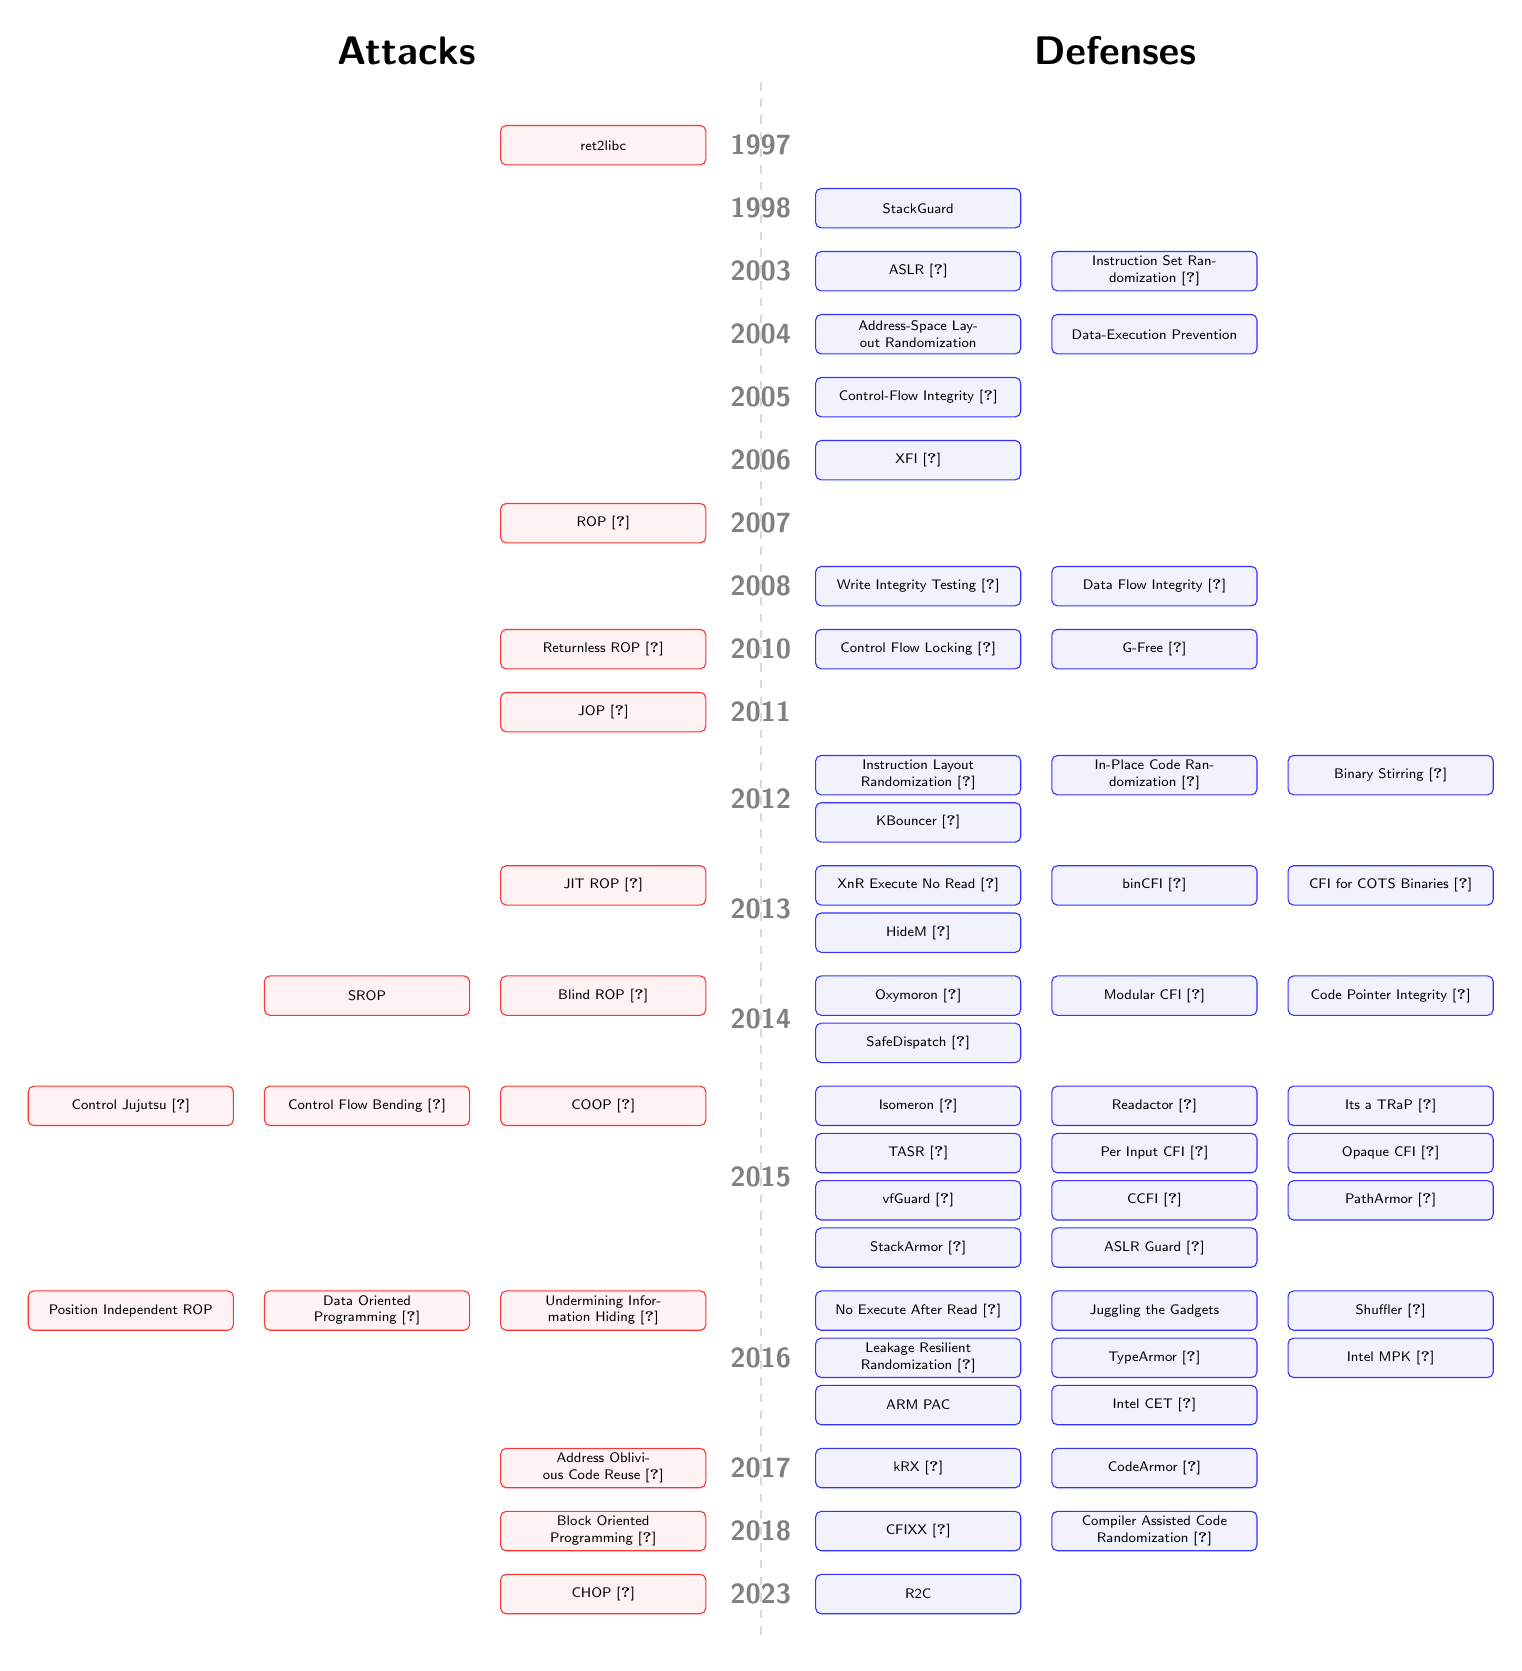
\begin{tikzpicture}[
  year node/.style={font=\bfseries\sffamily\color{gray}, align=center, inner sep=2pt},
  attack node/.style={draw=red!80, fill=red!5, rounded corners=2pt, font=\tiny\sffamily, align=center, minimum width=2.6cm, minimum height=0.5cm, inner sep=1.5pt, text width=2.5cm},
  defense node/.style={draw=blue!80, fill=blue!5, rounded corners=2pt, font=\tiny\sffamily, align=center, minimum width=2.6cm, minimum height=0.5cm, inner sep=1.5pt, text width=2.5cm},
  spine/.style={thick, gray!30, dashed}
]
  \node[font=\Large\bfseries\sffamily] at (-4.5, 1.2) {Attacks};
  \node[font=\Large\bfseries\sffamily] at (4.5, 1.2) {Defenses};
  % Year 1997
  \node[year node] (Y1997) at (0, 0.00) {1997};
  \node[attack node] at (-2.00, 0.00) {ret2libc};
  % Year 1998
  \node[year node] (Y1998) at (0, -0.80) {1998};
  \node[defense node] at (2.00, -0.80) {StackGuard};
  % Year 2003
  \node[year node] (Y2003) at (0, -1.60) {2003};
  \node[defense node] at (2.00, -1.60) {ASLR~\cite{PaXTeam2003}};
  \node[defense node] at (5.00, -1.60) {Instruction Set Randomization~\cite{boyd2010}};
  % Year 2004
  \node[year node] (Y2004) at (0, -2.40) {2004};
  \node[defense node] at (2.00, -2.40) {Address-Space Layout Randomization};
  \node[defense node] at (5.00, -2.40) {Data-Execution Prevention};
  % Year 2005
  \node[year node] (Y2005) at (0, -3.20) {2005};
  \node[defense node] at (2.00, -3.20) {Control-Flow Integrity~\cite{Abadi2005}};
  % Year 2006
  \node[year node] (Y2006) at (0, -4.00) {2006};
  \node[defense node] at (2.00, -4.00) {XFI~\cite{Erlingsson2006}};
  % Year 2007
  \node[year node] (Y2007) at (0, -4.80) {2007};
  \node[attack node] at (-2.00, -4.80) {ROP~\cite{Shacham2007}};
  % Year 2008
  \node[year node] (Y2008) at (0, -5.60) {2008};
  \node[defense node] at (2.00, -5.60) {Write Integrity Testing~\cite{Akritidis2008}};
  \node[defense node] at (5.00, -5.60) {Data Flow Integrity~\cite{castro2006}};
  % Year 2010
  \node[year node] (Y2010) at (0, -6.40) {2010};
  \node[attack node] at (-2.00, -6.40) {Returnless ROP~\cite{checkoway2010}};
  \node[defense node] at (2.00, -6.40) {Control Flow Locking~\cite{Bletsch2011b}};
  \node[defense node] at (5.00, -6.40) {G-Free~\cite{Onarlioglu2010}};
  % Year 2011
  \node[year node] (Y2011) at (0, -7.20) {2011};
  \node[attack node] at (-2.00, -7.20) {JOP~\cite{Bletsch2011a}};
  % Year 2012
  \node[year node] (Y2012) at (0, -8.30) {2012};
  \node[defense node] at (2.00, -8.00) {Instruction Layout Randomization~\cite{Hiser2012}};
  \node[defense node] at (5.00, -8.00) {In-Place Code Randomization~\cite{Pappas2012a}};
  \node[defense node] at (8.00, -8.00) {Binary Stirring~\cite{Wartell2012}};
  \node[defense node] at (2.00, -8.60) {KBouncer~\cite{Pappas2013b}};
  % Year 2013
  \node[year node] (Y2013) at (0, -9.70) {2013};
  \node[attack node] at (-2.00, -9.40) {JIT ROP~\cite{Snow2013}};
  \node[defense node] at (2.00, -9.40) {XnR Execute No Read~\cite{Backes2013}};
  \node[defense node] at (5.00, -9.40) {binCFI~\cite{zhang2013}};
  \node[defense node] at (8.00, -9.40) {CFI for COTS Binaries~\cite{zhang2013}};
  \node[defense node] at (2.00, -10.00) {HideM~\cite{Goktas2016b}};
  % Year 2014
  \node[year node] (Y2014) at (0, -11.10) {2014};
  \node[attack node] at (-2.00, -10.80) {Blind ROP~\cite{Bittau2014a}};
  \node[attack node] at (-5.00, -10.80) {SROP};
  \node[defense node] at (2.00, -10.80) {Oxymoron~\cite{Backes2014f}};
  \node[defense node] at (5.00, -10.80) {Modular CFI~\cite{niu2014a}};
  \node[defense node] at (8.00, -10.80) {Code Pointer Integrity~\cite{Kuznetsov2014}};
  \node[defense node] at (2.00, -11.40) {SafeDispatch~\cite{jang2014}};
  % Year 2015
  \node[year node] (Y2015) at (0, -13.10) {2015};
  \node[attack node] at (-2.00, -12.20) {COOP~\cite{Schuster2015a}};
  \node[attack node] at (-5.00, -12.20) {Control Flow Bending~\cite{Carlini2015a}};
  \node[attack node] at (-8.00, -12.20) {Control Jujutsu~\cite{Evans2015a}};
  \node[defense node] at (2.00, -12.20) {Isomeron~\cite{Davi2015}};
  \node[defense node] at (5.00, -12.20) {Readactor~\cite{Crane2015}};
  \node[defense node] at (8.00, -12.20) {Its a TRaP~\cite{Crane2015b}};
  \node[defense node] at (2.00, -12.80) {TASR~\cite{bigelow2015}};
  \node[defense node] at (5.00, -12.80) {Per Input CFI~\cite{Niu2015}};
  \node[defense node] at (8.00, -12.80) {Opaque CFI~\cite{Mohan2015}};
  \node[defense node] at (2.00, -13.40) {vfGuard~\cite{Prakash2015}};
  \node[defense node] at (5.00, -13.40) {CCFI~\cite{Mashtizadeh2015}};
  \node[defense node] at (8.00, -13.40) {PathArmor~\cite{Goktas2016b}};
  \node[defense node] at (2.00, -14.00) {StackArmor~\cite{Chen2015c}};
  \node[defense node] at (5.00, -14.00) {ASLR Guard~\cite{Lu2015}};
  % Year 2016
  \node[year node] (Y2016) at (0, -15.40) {2016};
  \node[attack node] at (-2.00, -14.80) {Undermining Information Hiding~\cite{Goktas2016}};
  \node[attack node] at (-5.00, -14.80) {Data Oriented Programming~\cite{Hu2016}};
  \node[attack node] at (-8.00, -14.80) {Position Independent ROP};
  \node[defense node] at (2.00, -14.80) {No Execute After Read~\cite{Werner2016}};
  \node[defense node] at (5.00, -14.80) {Juggling the Gadgets};
  \node[defense node] at (8.00, -14.80) {Shuffler~\cite{WilliamsKing2016}};
  \node[defense node] at (2.00, -15.40) {Leakage Resilient Randomization~\cite{Braden2016}};
  \node[defense node] at (5.00, -15.40) {TypeArmor~\cite{VanderVeen2015b}};
  \node[defense node] at (8.00, -15.40) {Intel MPK~\cite{Wahbe1993}};
  \node[defense node] at (2.00, -16.00) {ARM PAC};
  \node[defense node] at (5.00, -16.00) {Intel CET~\cite{IntelCET}};
  % Year 2017
  \node[year node] (Y2017) at (0, -16.80) {2017};
  \node[attack node] at (-2.00, -16.80) {Address Oblivious Code Reuse~\cite{Rudd2017}};
  \node[defense node] at (2.00, -16.80) {kRX~\cite{Pomonis2019}};
  \node[defense node] at (5.00, -16.80) {CodeArmor~\cite{Chen2017a}};
  % Year 2018
  \node[year node] (Y2018) at (0, -17.60) {2018};
  \node[attack node] at (-2.00, -17.60) {Block Oriented Programming~\cite{Ispoglou2018}};
  \node[defense node] at (2.00, -17.60) {CFIXX~\cite{Burow2018CFIXX}};
  \node[defense node] at (5.00, -17.60) {Compiler Assisted Code Randomization~\cite{Koo2018}};
  % Year 2023
  \node[year node] (Y2023) at (0, -18.40) {2023};
  \node[attack node] at (-2.00, -18.40) {CHOP~\cite{duta2023}};
  \node[defense node] at (2.00, -18.40) {R2C};
  \draw[spine] (0, 0.8) -- (0, -19.00);
\end{tikzpicture}
}
